\subsection{ADC DC Offset} \label{subsec:ADCDCOffset}
The LTC2311 ADCs can sample signals in the range $GNDA < V_{IN} < V_{REF}$. The input signals are sinusoidal and is expected to swing below GNDA, so a \SIQ{2.5}{\volt} DC offset is added to the inputs so the signals stay in the specified range. The \SIQ{2.5}{\volt} offset is created by a voltage divider that is being tapped off from the \SIQ{5}{\volt} ADC reference as shown on figure \refq{fig_7_1_3_ADC2.5VOFFSET}.

\begin{figure}[H]
    \centering
    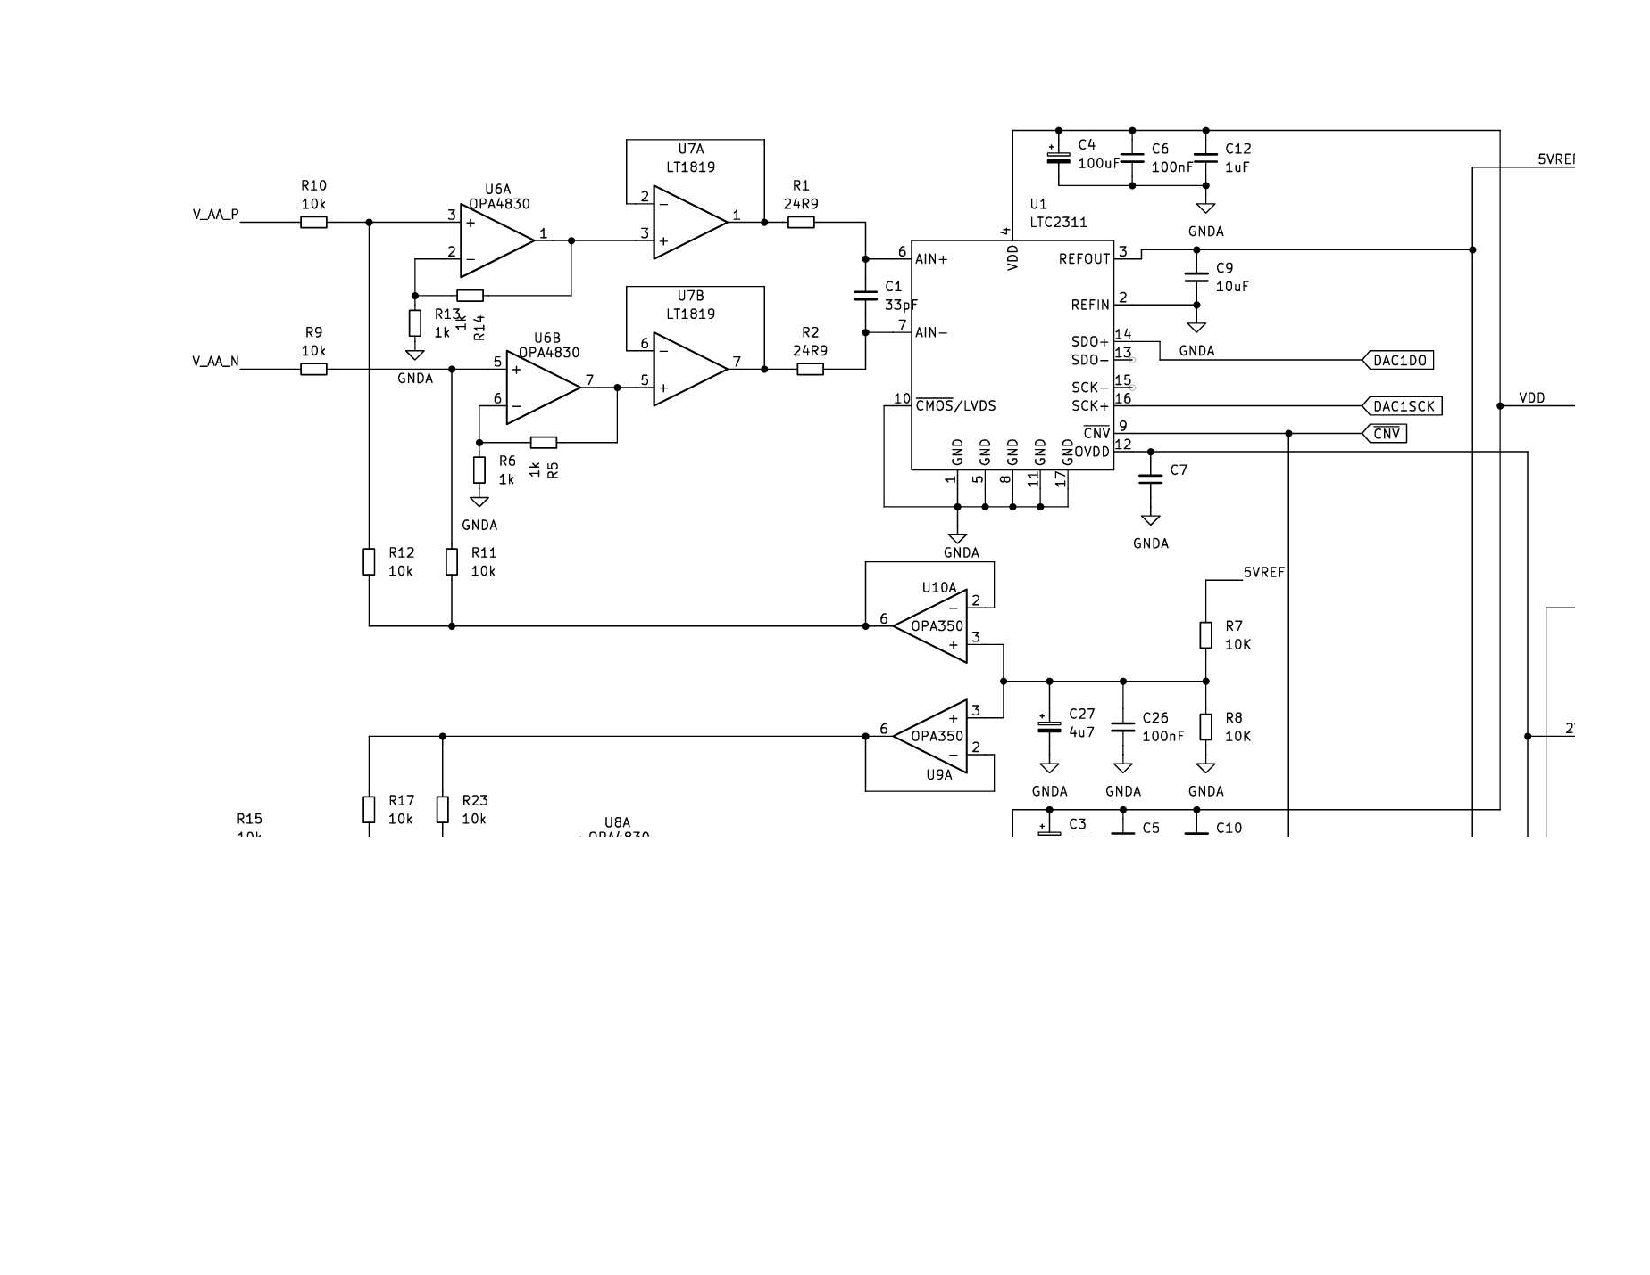
\includegraphics[clip, trim=0 200 0 0, width=1\textwidth]{Sections/7_SystemDesign/Figures/7_1_3_DCOFFSET.pdf}
    \caption{The 5V reference is fed into the R7, R8 voltage divider to create a 2.5V reference that is used as input to the U10A and U9A buffers. Only the U10A signal path is considered here as the U9A path is identical. This buffer is feeding the input of the summation amplifiers U6A and U6B.}
    \label{fig_7_1_3_ADC2.5VOFFSET}
\end{figure}

A low pass filter was added to the input of the buffers. Assuming an infinite input impedance of the buffer U10A, U9A and zero output impedance from the 5V reference source, the voltage divider will form an additional simple 1-pole RC filter with the C27, C26 capacitors with a cut-off close to DC as shown in eq \refq{eq:7_1_3_SimplePole}.

\begin{equation}\label{eq:7_1_3_SimplePole}
    f_{c} = \frac{1}{2\pi (R_7^{-1} + R_8^{-1})^{-1}(C_{27}+C_{28})} \approx 6.63 Hz 
\end{equation}

The output of buffer U10A feeds into the summation points at the non-inverting inputs of U6A and U7B through R12 and R11. Assuming an infinite input impedance of U6A and U6B and zero output impedance of the V\_AA\_P, V\_AA\_N signal sources, the DC voltage in the summation point will be set by a simple voltage divider and will be \SIQ{1.25}{\volt} as shown in equation \refq{eq:7_1_3_InputVolt}.

\begin{equation}\label{eq:7_1_3_InputVolt}
    V_{IN6A6B} = V_{O10A} \cdot \frac{R_{10}}{R_{10}+R_{12}} = 1.25V
\end{equation}

The two amplifiers are, once again, identical. U6A and U6B have a gain of $A_V = \frac{R_{14}}{R_{13}} + 1 =  2$ in order to produce the final \SIQ{2.5}{\volt} DC offset that the ADC needs. 

